\documentclass[UTF8]{ctexart}
\usepackage{subfigure}
\usepackage{caption}
\usepackage{amsmath}
\usepackage{geometry}
\usepackage{graphicx}
\usepackage{gensymb}
\usepackage{wrapfig}
\usepackage{titlesec}
\usepackage{float}
\usepackage{diagbox}
\usepackage{fancyhdr}
\pagestyle{plain}
\geometry{a4paper,scale=0.8}
\CTEXsetup[format+={\raggedright}]{section} 
\title{量统2018-2019郭永期末}
\author{Deschain}
\titlespacing*{\section}
{0pt}{0pt}{0pt}
\titlespacing*{\subsection}
{0pt}{0pt}{0pt}
\titlespacing*{\paragraph}
{0pt}{0pt}{0pt}
\titlespacing*{\subparagraph}
{0pt}{0pt}{0pt}
\titleformat*{\section}{\normalsize}
\begin{document}
\maketitle
\section*{一、(本题20分)如果不考虑原子内电子的运动,双原子理想气体分子的能量为
  $\varepsilon_i=\varepsilon_j^t+\varepsilon_l^r+\varepsilon_n^\nu$,包括分子平动能
  $\varepsilon_j^t$、转动能$\varepsilon_l^r$和振动能$\varepsilon_n^\nu$,简并度分别为
  $g_j^t,g_l^r,g_n^\nu$。解答下列问题:}
1.给出双原子理想气体分子的配分函数与平动配分函数、转动配分函数和振动配分函数之间的关系;\\
设双原子气体分子的配分函数为$z$,平动、转动、振动的配分函数依次为$z^t,z^r,z^\gamma$,则
$z=z^tz^rz^\gamma$\\
2.计算N个双原子理想气体分子质心平动的内能、定容热容量及压强;
\begin{equation*}
  \begin{aligned}
     & g(\varepsilon)=\frac{2\pi VJ}{h^3}(2m)^\frac{3}{2}\sqrt{\varepsilon}d\varepsilon,\quad
    z^t=\int_0^\infty g(\varepsilon)e^{-\beta\varepsilon}d\varepsilon
    =V(\frac{2\pi m}{\beta h^2})^\frac{3}{2}                                                  \\
     & \overline{E}^t=-N\frac{\partial lnz}{\partial\beta}=\frac{3}{2}NkT,\quad
    C_V^t=\frac{\partial\overline{E}}{\partial T}=\frac{3}{2}Nk,\quad                         \\
     & P^t=\frac{N}{\beta}\frac{\partial lnz^r}{\partial V}=0
  \end{aligned}
\end{equation*}
3.双原子分子中两原子的相对振动可以看成是质量为$\mu(=\frac{m_1m_2}{m_1+m_2})$的线性振子
作简谐振动,计算振动能和振动热容量,解释为什么在常温下振动自由度可以视为“冻结”自由度?
\begin{equation*}
  \begin{aligned}
     & \varepsilon_n=(n+\frac{1}{2})h\nu,\quad\quad g_n=1    \\
     & z^\nu=\sum e^{-\beta\varepsilon_n}
    =\frac{e^{-\frac{\beta h\nu}{2}}}{1-e^{-\beta h\nu}}     \\
     & \overline{E}^\nu=-N\frac{\partial lnz}{\partial\beta}
    =Nh\nu(\frac{1}{2}+\frac{1}{e^{\beta h\nu}-1})           \\
     & C_V=\frac{\partial\overline{E}}{\partial T}
    =Nk(\beta h\nu)^2\frac{e^{\beta h\nu}}{(e^{\beta h\nu}-1)^2}
  \end{aligned}
\end{equation*}
常温下$\beta h\nu>>1$,$C_V\approx Nk(\beta h\nu)^2e^{-\beta h\nu}<<Nk$,所以振动自由度是冻结的。\\
4.讨论平动及振动对气体压强的贡献。
\begin{equation*}
  P^\nu=\frac{N}{\beta}\frac{\partial lnz^\nu}{\partial V}=0
\end{equation*}
振动对压强无贡献。
\section*{二、(本题20分)定域系统中的粒子在严格的量子力学意义上是全同的,但各个粒子各自
  局限在一定范围内运动,因而可以根据位置加以区分。考虑一个由N个粒子组成,具有能量E和体积V的
  孤立定域系统,设$\varepsilon_i,g_i,n_i$分别是单粒子能级i的能量、简并度及粒子分布数。
  解答下列问题:}
1.在什么情况下该定域系统可视为近独立粒子系统?\\
系统的粒子间的相互作用的平均能量远远小于单个粒子的平均能量。\\
2.直接写出该定域系统中任意一组分布$\{n_i\}$所包含的微观状态数。\\
\begin{equation*}
  W\{n_i\}=N!\prod\limits_i\frac{g_i^{n_i}}{n_i!}
\end{equation*}
3.解释什么是等几率原理?基于该原理并采用Lanrange待定乘子法,导出Boltzmann分布
$n_i=g_ie^{-\alpha-\beta\varepsilon}\quad(i=1,2,\cdots)$,进而解释$\alpha$、$\beta$
的物理意义及该分布的含义。\\
等几率原理:处于平衡态的孤立系统,各个微观态出现的几率相等。
\begin{equation*}
  \begin{aligned}
     & W\{n_i\}\approx N^N\prod\limits_i\frac{g_i^{n_i}}{n_i!},\quad\quad
    ln(W\{n_i\})=NlnN+\sum n_ilng_i-\sum n_ilnn_i                                       \\
     & F(n_i)=ln(W\{n_i\})+\alpha(N-\sum n_i)+\beta(E-\sum n_i\varepsilon_i)            \\
     & \frac{\partial F}{\partial n_i}=lng_i-1-lnn_i-\alpha-\beta\varepsilon_i=0        \\
     & n_i=g_ie^{-\alpha-\beta\varepsilon_i-1}\approx g_ie^{-\alpha-\beta\varepsilon_i}
    \alpha=-\frac{\mu}{kT},\quad\quad \beta=-\frac{1}{kT}                               \\
  \end{aligned}
\end{equation*}
物理意义:$\mu$是化学势,k是Boltzmann常数,T是热力学温度。\\
含义:定域粒子系统处于平衡态的分布,给出了处于平衡态时对能级$\varepsilon_i$分布的粒子数。\\
4.Bose分布与Fermi分布在什么条件下趋于半经典分布$n_i=g_ie^{-\alpha-\beta\varepsilon_i}$?
半经典分布与Boltzmann分布完全相同,但统计不同,给出两者的主要区别。\\
参考公式:Stirling公式$N!\approx N^Ne^{-N}\quad(N>>1)$\\
(1)$e^\alpha>>1$\\
(2)半经典分布中,粒子不可区分,$W\{n_i\}=\prod\limits_i\frac{g_i^{n_i}}{n_i!}$\\
Boltzmann分布中,粒子可区分,$W\{n_i\}=N!\prod\limits_i\frac{g_i^{n_i}}{n_i!}$\\
\section*{三、(本题20分)金属固体中的电子可看作三维自由电子气体。解答下列问题:}
1.电子气体满足何种分布?画草图并解释$T=0K$时分布函数的特点,导出费米能的表达式,进而说明
费米能的物理含义;\\
\subsection*{}
\begin{wrapfigure}{r}{3cm}
  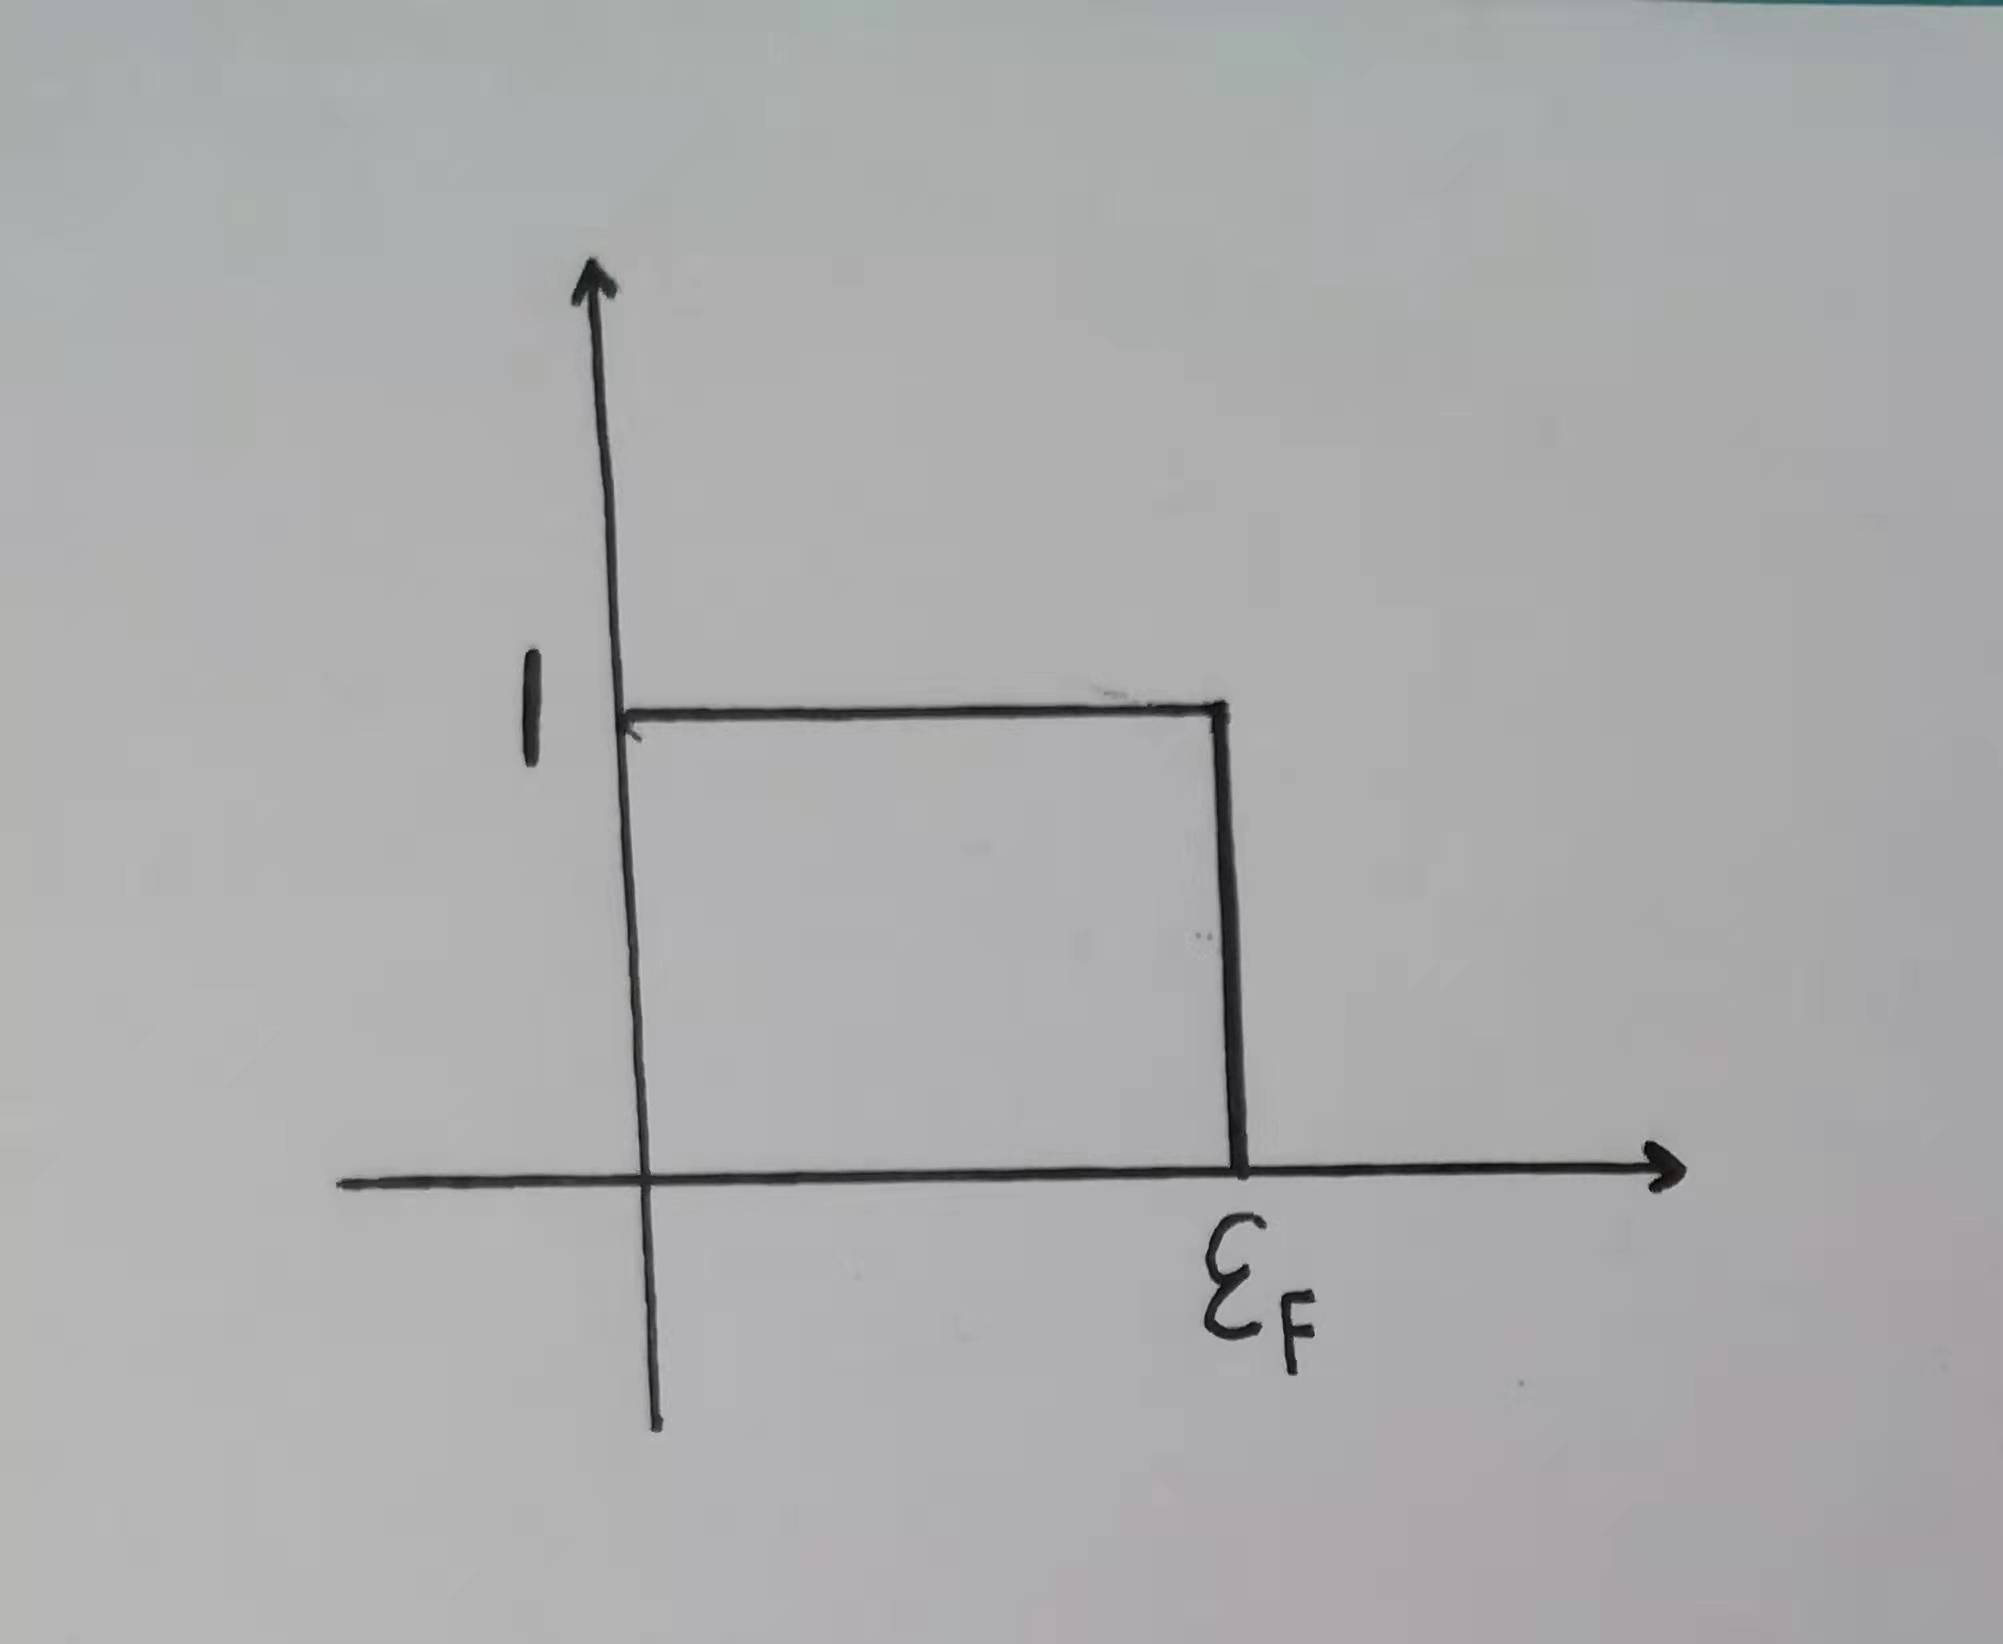
\includegraphics[width=3cm]{3_1.jpg}
\end{wrapfigure}
费米分布。\\
$T=0K$时,低于$\varepsilon_F$的能级完全填满,高于$\varepsilon_F$的能级完全空着。\\
\subsection*{}
\begin{equation*}
  \begin{aligned}
     & g(\varepsilon)=\frac{2\pi VJ}{h^3}(2m)^\frac{3}{2}\sqrt{\varepsilon}
    = CV\sqrt{\varepsilon}.\quad\quad
    C =\frac{2\pi J}{h^3}(2m)^\frac{3}{2}                                   \\
     & N=\int_0^{\varepsilon_F}g(\varepsilon)d\varepsilon
    =\frac{2}{3}CV\varepsilon_F^\frac{3}{2},\quad\quad
    \varepsilon_F=\frac{h^2}{2m}(\frac{3N}{4\pi JV})^\frac{2}{3}
    =\frac{h^2}{2m}(\frac{3N}{8\pi V})^\frac{2}{3}
  \end{aligned}
\end{equation*}
$\varepsilon_F$的物理意义,$T=0K$时电子占据态的最高能级,是电子占据态与非占据态的分界面。\\
2.研究表明低温下金属的定容热容量为$C_V=\gamma T+AT^3$,其中第一项为自由电子的贡献,第二项是
晶格振动的贡献。简单论证电子对热容量的贡献正比于温度T,直接指出第二项是由何种著名晶格振动模型
得出的结果?\\
\begin{equation*}
  \overline{E}\approx\frac{2Nk^2T^2}{\varepsilon_F},\quad\quad
  C_V=\frac{\partial\overline{E}}{\partial T}=\frac{4Nk^2T}{\varepsilon_F}
\end{equation*}
Einstein的晶格振动模型。\\
3.如果金属薄膜中的自由电子近似地看作在二维平面上的运动,面密度为n。求$T=0K$时二维电子的费米能
量、内能及简并压。
\begin{equation*}
  \begin{aligned}
     & \Omega(\varepsilon)=2\pi Sm\varepsilon,\quad\quad
    g(\varepsilon)=\frac{4\pi Sm}{h^2}                                                  \\
     & N=\int_0^{\varepsilon_F}\frac{4\pi Sm}{h^2}d\varepsilon
    =\frac{4\pi Sm}{h^2}\varepsilon_F,\quad\quad
    \varepsilon_F=\frac{nh^2}{4\pi m}                                                   \\
     & \overline{E}_0=\int_0^{\varepsilon_F}\frac{4\pi Sm}{h^2}\varepsilon d\varepsilon
    =\frac{n^2h^2S}{8\pi m},\quad\quad
    P=\frac{\overline{E}}{S}=\frac{n^2h^2}{8\pi m}
  \end{aligned}
\end{equation*}
\section*{四、(本题20分)考虑一磁场中由可区分的自旋量子数为$\frac{1}{2}$的原子构成的刚性晶
  格,原子的自旋磁矩为$\vec\mu$,自旋相对于外磁场$\vec H$有平行和反平行两个态,此系统的温度为T。
  系统服从玻尔兹曼分布。解答下列问题:}
1.一个原子处于自旋平行态与反自旋平行态能量及相应几率。\\
2.此系统的平均总磁矩、磁化强度及熵。\\
3.高温弱场和低温强场时平均总磁矩的极限表达式,给出达到饱和磁化的条件。\\
\section*{五、(本题20分)理想玻色气体的粒子数、温度及化学势分别为N、T和$\mu$;单粒子基态能级
  的能量与分布数分别为$\varepsilon_0$、$N_0$。解答下列问题:}
1.试根据玻色-爱因斯坦分布,证明理想玻色气体具有如下性质:
\begin{equation*}
  \begin{aligned}
     & (1)\lim_{T\to0K}N_0=N             \\
     & (2)\lim_{T\to0K}\mu=\varepsilon_0 \\
  \end{aligned}
\end{equation*}
\newline
\begin{equation*}
  \begin{aligned}
     & n_i=\frac{g_i}{e^\frac{\varepsilon-\mu}{kT}-1}>0,\quad\quad
    \mu<\varepsilon_i,\quad\quad\mu<\varepsilon_0                      \\
     & \lim_{T\to0}N_{i>0}=0,\quad\quad\lim_{T\to0}N_0=N               \\
     & \lim_{T\to0}\frac{\varepsilon_0-\mu}{kT}=\frac{0}{0},\quad\quad
    \lim_{T\to0}\mu=\varepsilon_0
  \end{aligned}
\end{equation*}
2.简要解释玻色-爱因斯坦凝聚现象及因何称这种凝聚是动量空间中的凝聚而非坐标空间中的凝聚?\\
当温度从$T_c$开始下降时,基态上的粒子数迅速增加,与总粒子数具有相同的量级。$T=0K$时,全部粒子
集中在基态上。\\
$\varepsilon_0$态上的粒子能量、动量、熵均为0。\\
3.考虑质量为m的N个无自旋玻色粒子的气体,封闭在温度为T的体积V中。\\
(1)求出作为单粒子能量$\varepsilon$函数的单粒子态密度$g(\varepsilon)$,并画出结果。\\
\begin{equation*}
  \begin{aligned}
     & \Omega(\varepsilon)=\int dxdydz\int dp_xdp_ydp_z=\frac{4\pi}{3}V(2m\varepsilon)\frac{3}{2} \\
     & g(\varepsilon)=\frac{J\Omega(\varepsilon)}{h^3d\varepsilon}
    =\frac{4\pi V(2m)^\frac{3}{2}\sqrt{\varepsilon}}{h^3}                                         \\
  \end{aligned}
\end{equation*}
\begin{figure}[H]
  \centering
  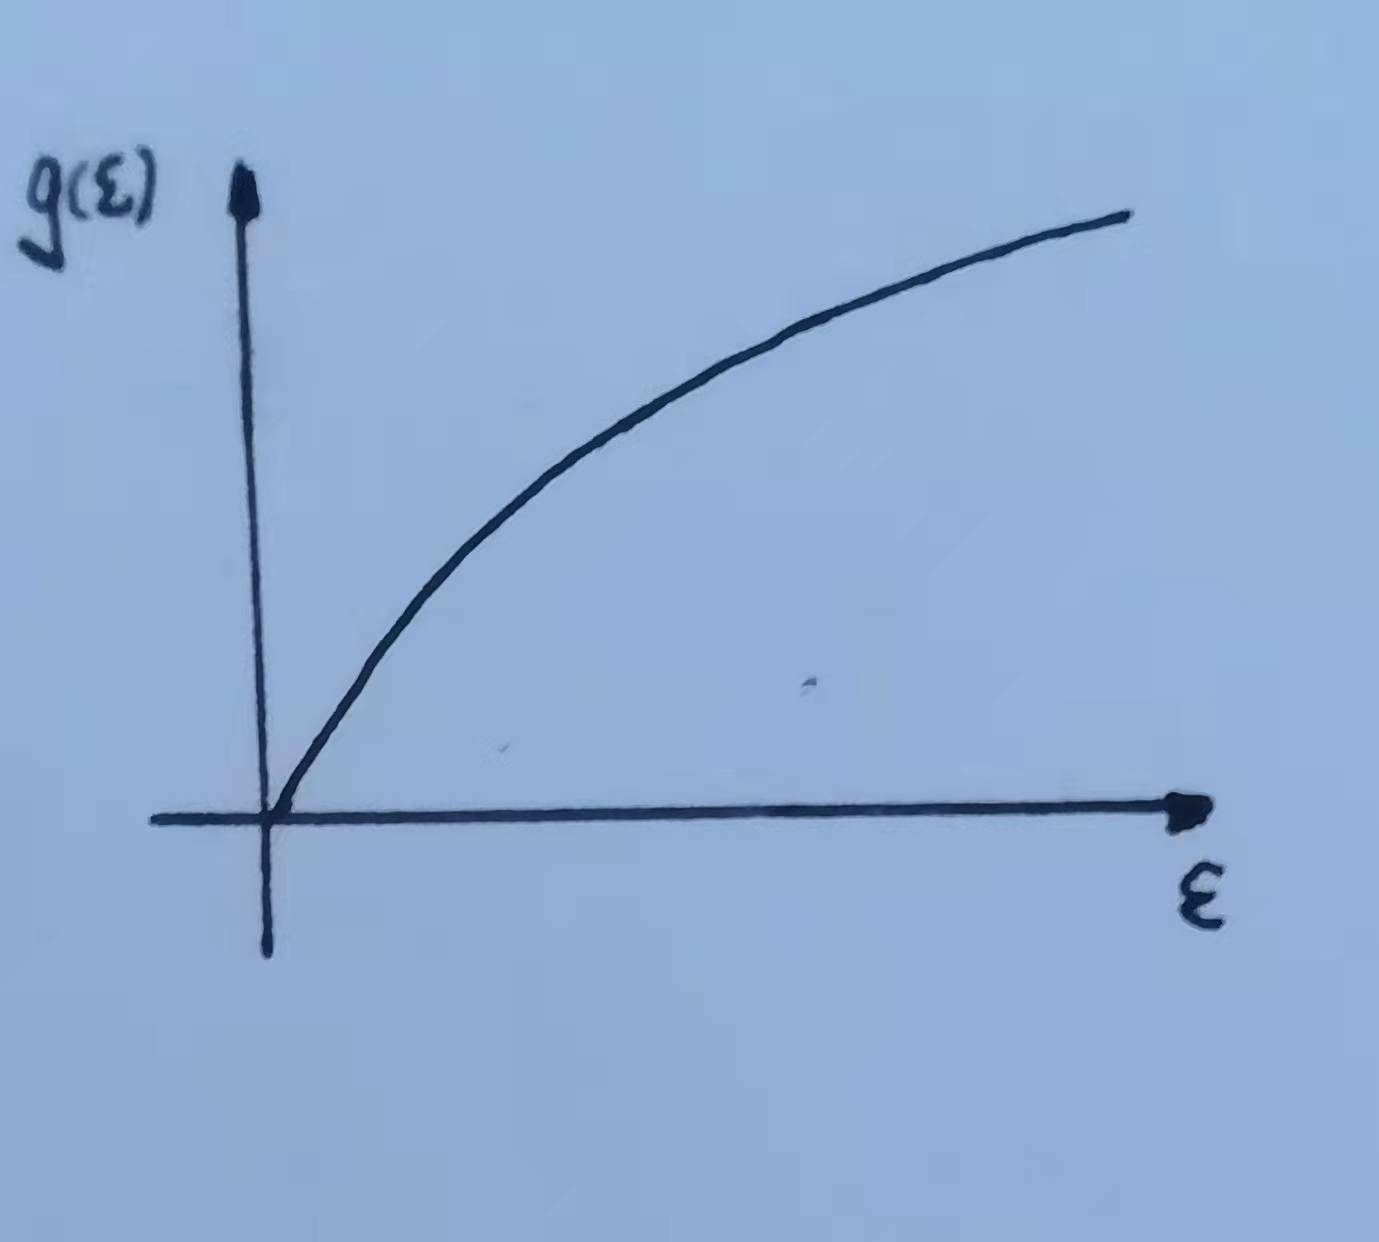
\includegraphics[width=4cm,height=4cm]{5_3_1.jpg}
\end{figure}
(2)写出作为$\varepsilon$、$T$和化学势$\mu(T)$函数的单量子态平均分布数,对一适当高的温度(即
玻色-爱因斯坦相变以上的温度),在(1)部分的图中画上这个函数并在$\varepsilon$轴上标明
$\varepsilon=\mu$的位置。
\begin{equation*}
  f_i=\frac{n_i}{g_i}=\frac{1}{e^{\alpha+\beta\varepsilon_i}-1}
  =\frac{1}{e^\frac{\varepsilon_i-\mu}{kT}-1}
\end{equation*}
\begin{figure}[H]
  \centering
  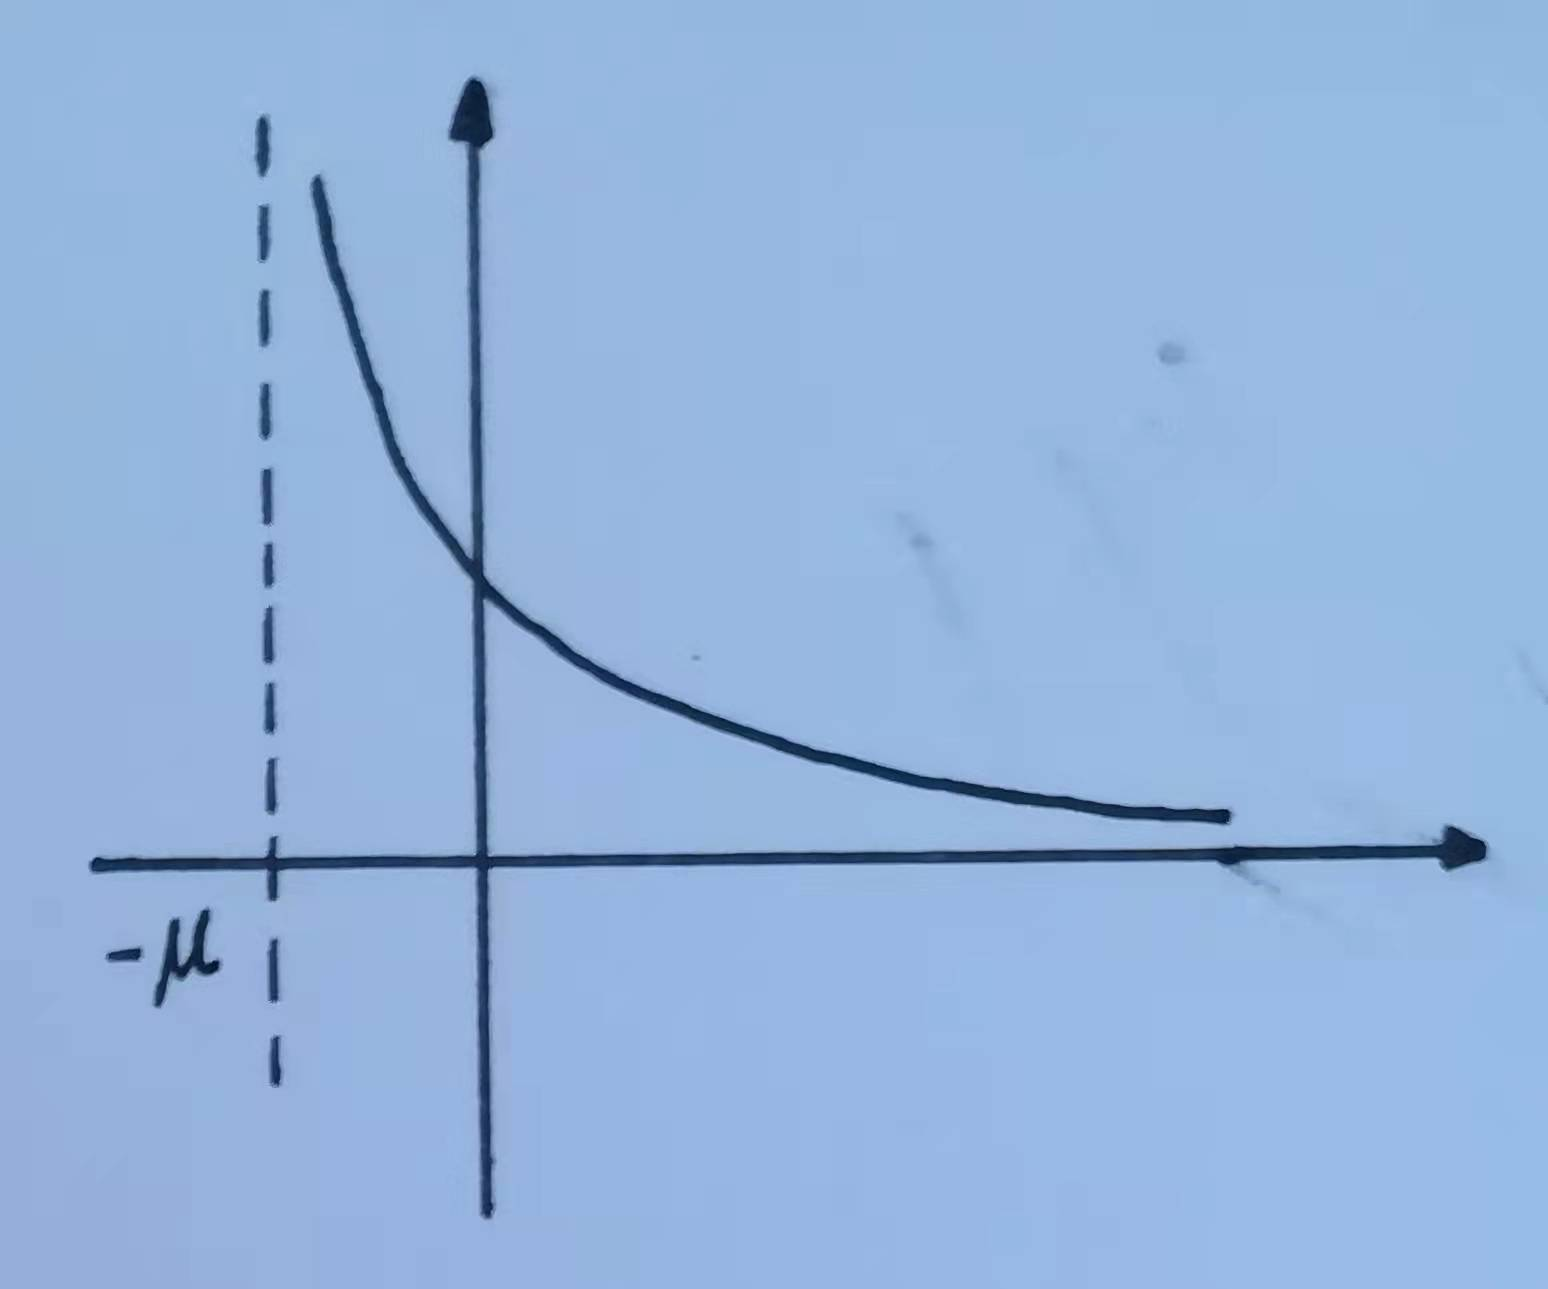
\includegraphics[width=4cm,height=4cm]{5_3_2.jpg}
\end{figure}
(3)对$T<T_c$($T_c$为临界温度),求这种气体的总能量$U(T,V)$的准确表达式,用无量纲积分表示。\\
参考公式:
\begin{equation*}
  \int_0^\infty\frac{\sqrt{x}dx}{e^x-1}=2.612\times\frac{\sqrt{\pi}}{2};\quad\quad
  \int_0^\infty\frac{x^\frac{3}{2}dx}{e^x-1}=\frac{3}{4}\sqrt{\pi}\times1.341
\end{equation*}
\begin{equation*}
  \begin{aligned}
     & g(\varepsilon)=\frac{2\pi V}{h^3}(2m)^\frac{3}{2}\sqrt{\varepsilon}          \\
     & \phi(\alpha,\beta,V)=g_0ln(1-e^{-\alpha})-\frac{2\pi J}{h^3}(2m)^\frac{3}{2}
    \int_0^\infty\sqrt{\varepsilon}ln(1-e^{-\alpha-\beta\varepsilon})d\varepsilon   \\
     & =-\frac{2\pi J}{h^3}(2m)^\frac{3}{2}
    \int_0^\infty\sqrt\varepsilon ln(1-e^{-\beta\varepsilon})d\varepsilon
    =1.341V(\frac{2\pi m}{\beta h^2})^\frac{3}{2}                                   \\
     & \overline{E}=-\frac{\partial\phi}{\partial\beta}
    =\frac{31.7V}{h^3}m^\frac{3}{2}(kT)^\frac{5}{2}
  \end{aligned}
\end{equation*}
\end{document}